%%
%%  Final Design and Engineering Specifications
%%

\subsubsection{Consolidated Sensors Interface}

\indent\indent To mitigate problems encountered by the first generation prototype, such as wires getting lose, losing connection, and in general a complex circuit with many components on separate breadboards, the second generation prototype opted to design a printed circuit board (PCB) [Fig. ~\ref{fig:PCB_top}] that consolidates all the sensors and connections on a single board that is mated to the RPi. This approach ensures all the sensors are properly seated and have a solid connection to the RPi. In addition, it removes a layer of complexity that is involved with maintaining the circuit on a breadboard with many wires. Moreover, this approach ensures that there is no latency over the I$^2$C lines since the connections are rather close to the I$^2$C bus on the RPi.

The PCB was designed to be used with female pins for the sensor inputs, this allows any faulty sensor to be swapped out with ease without the need to desolder and potentially harming the PCB. Furthermore, the PCB has multiple exposed GPIO pins for any future needs that users might need. The PCB was ground filled to prevent any short-circuits from occurring, however, it most be noted that the IMU placeholder has no ground fill underneath it, this was done to guarantee that the PCB won't interfere with the IMU's readings.

Lastly, the PCB is equipped with a rectifier diode to prevent any current flowing back into the RPi's GPIO pins and potentially damaging it. In addition to the diode, a $10\mu F$ capacitor was placed near the power line connecting the sensors to prevent any power fluctuations and spikes that might generate noisy signals.

\begin{figure}[H]
  \centering
  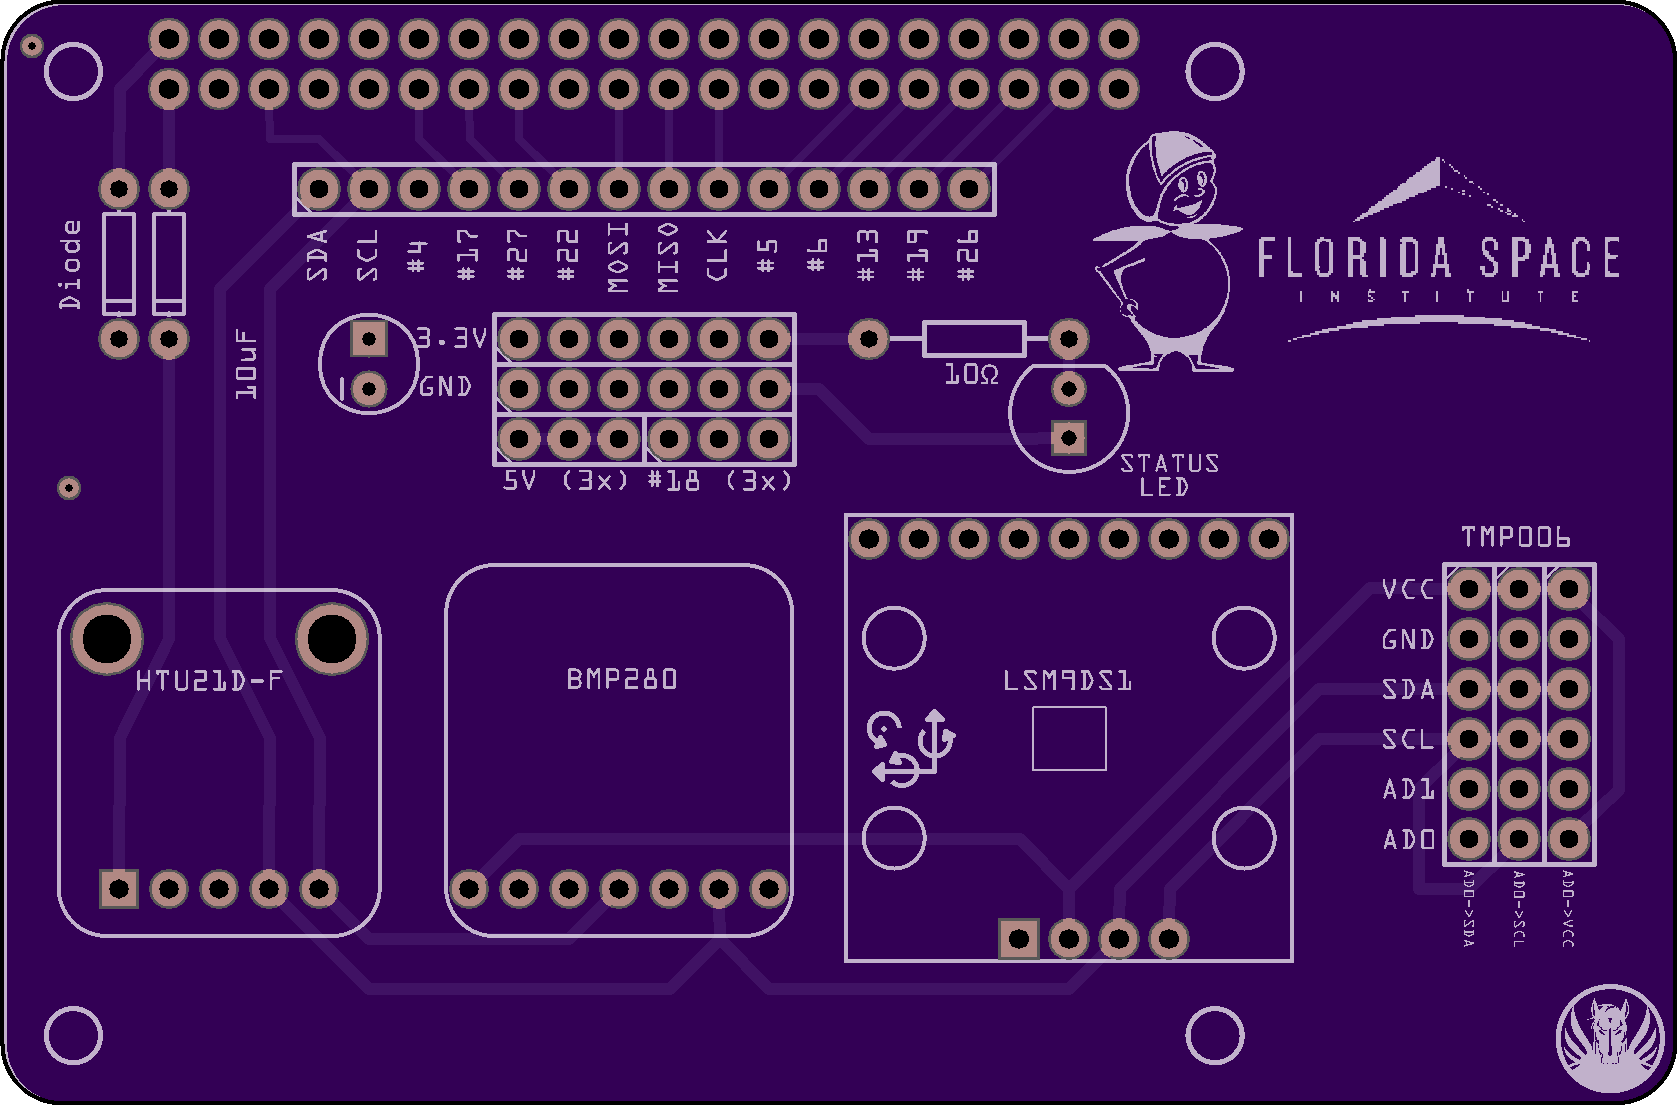
\includegraphics[width=0.75\linewidth]{Controls/PCB_top.png}
  \caption{\label{fig:PCB_top}PCB Top Layer} 
\end{figure}

\begin{figure}[H]
  \centering
  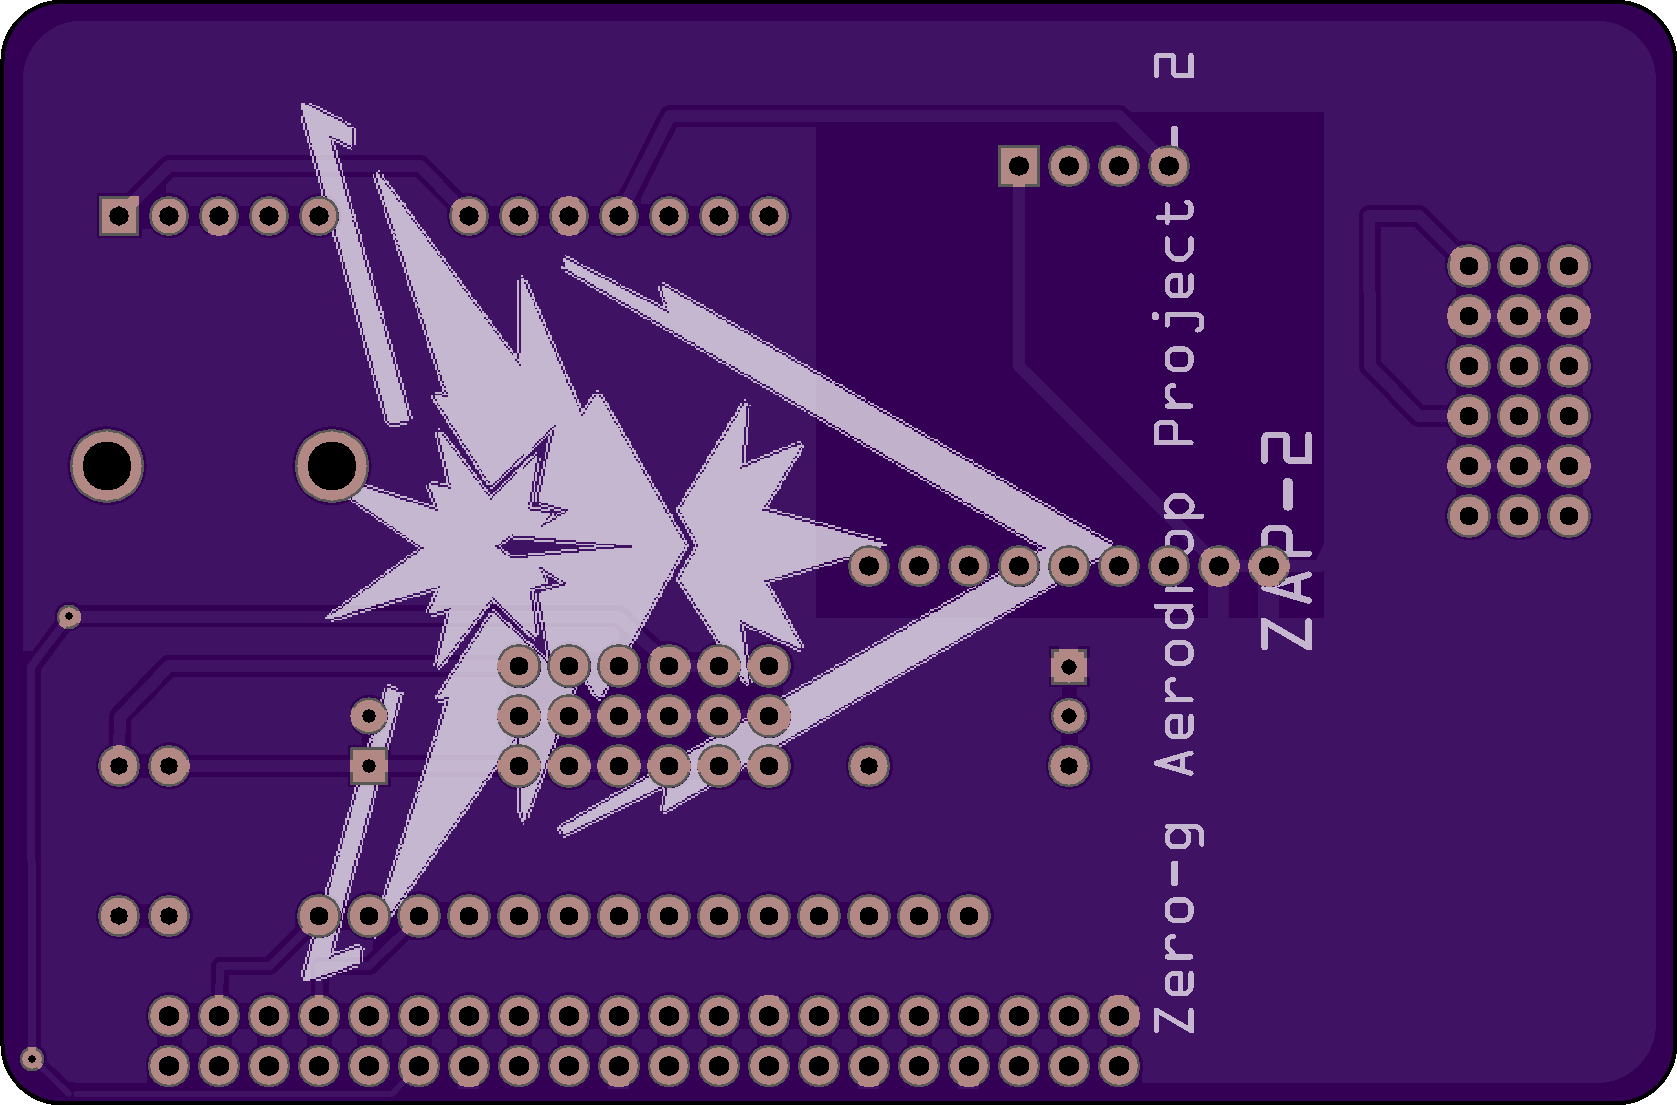
\includegraphics[width=0.75\linewidth]{Controls/PCB_bottom.png}
  \caption{\label{fig:PCB_bottom}PCB Bottom Layer}
\end{figure}